\chapter{System Architectural Design by DFD}
\section{Architectural Diagram}
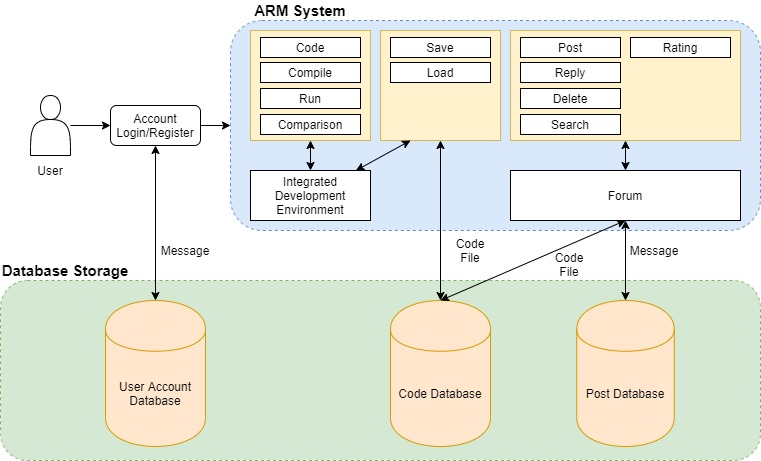
\includegraphics[scale=0.5]{Doc/Pics/architectural_diagram}
\newpage
\section{System Components}
\begin{enumerate}
	\item Personal Account System: Users Information are stored into the user database. Based on current design, users are classified into 3 class, normal user, student and teacher. They have no differences in this phase.
	\item Forum System: Posts are stored into the post database. List of post threads created by users, allows users to post and comment with thier source code. Users' posts can be searched and display to other users.
	\item Code Running System: Source code are stored into the code database. Source code created by users can be compiled, saved and load. Compiled program can be executed and its output will be shown.
\end{enumerate}
\section{Database}
\begin{enumerate}
	\item User Account Database includes username, account password, account type, extra permission of the account for teachers and student users to access posts only available to the class.
	\item Post Database includes posts contents (contents, author, reply, source code linkage, permission) and access frequencies of posts.
  \item Code Database includes source code file, author of the code, filename.
\end{enumerate}
\section{Data Flow Diagram(DFD)}
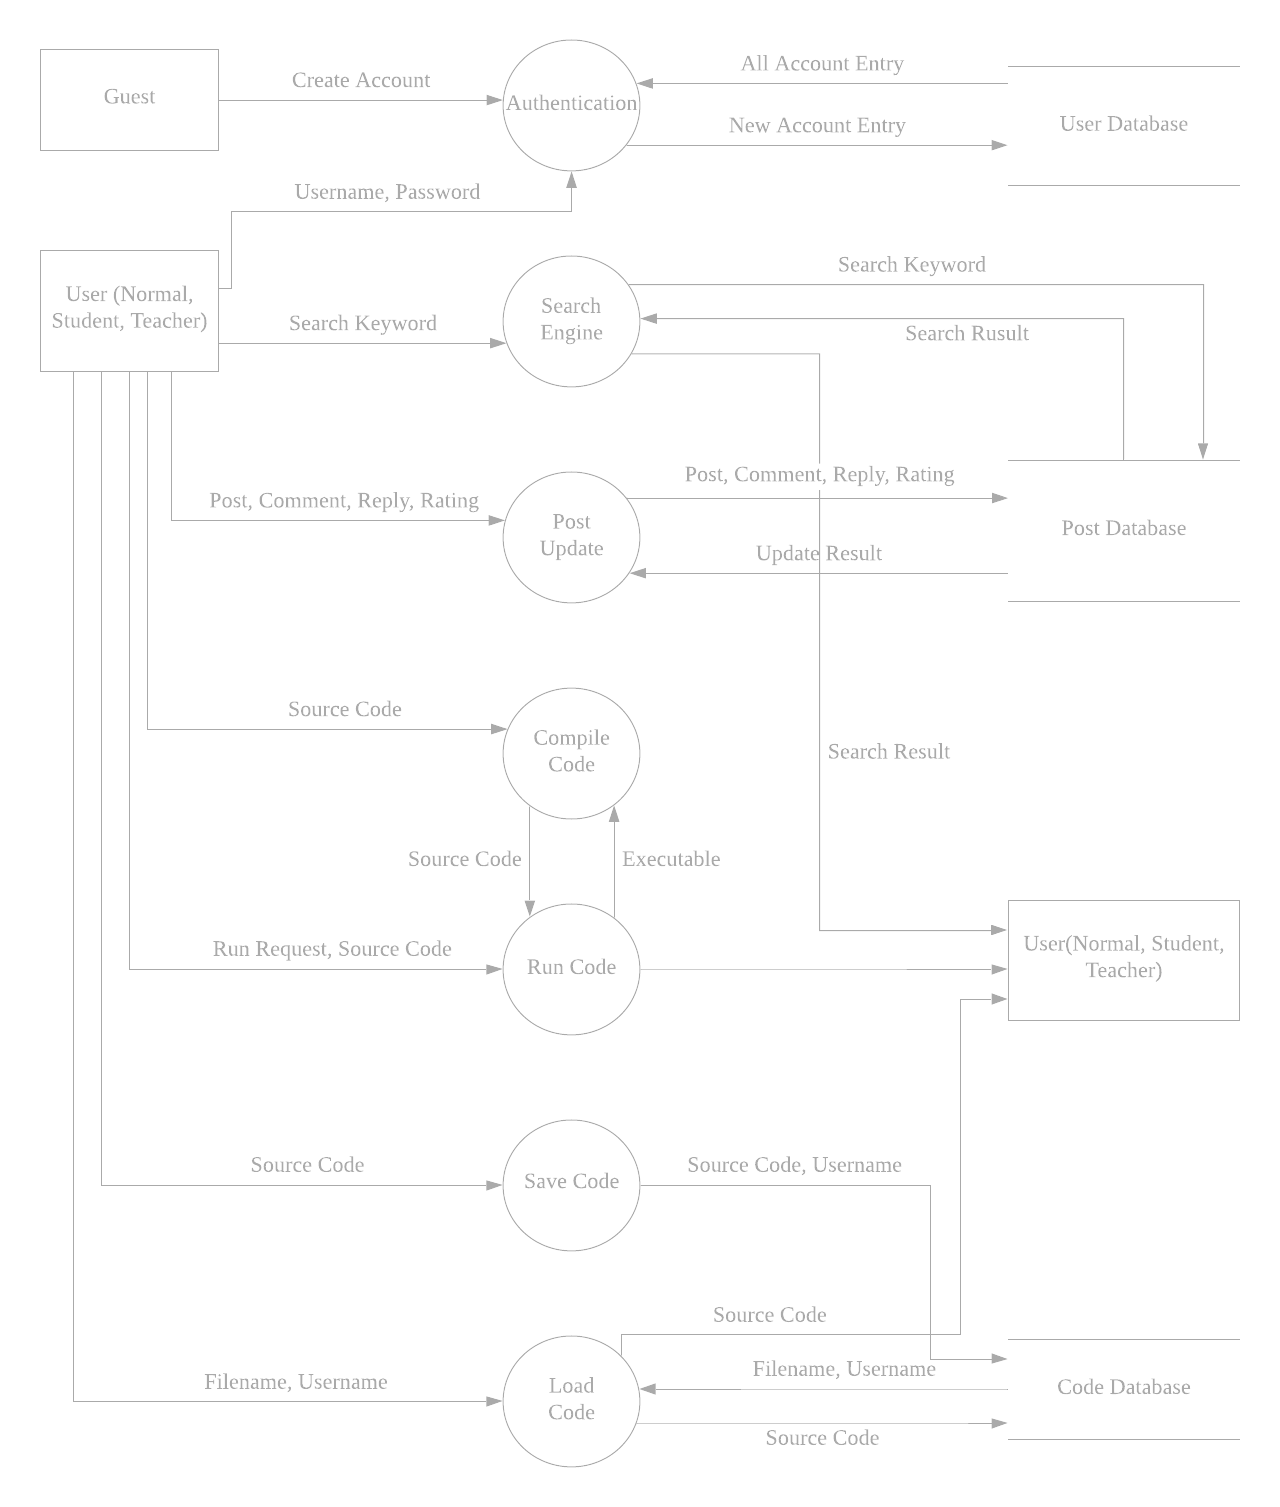
\includegraphics[scale=0.35]{Doc/Pics/dataflow_diagram}
